\documentclass[12pt]{article} 
%DIF LATEXDIFF DIFFERENCE FILE
%DIF DEL ms.tex      Wed Aug 10 17:58:00 2016
%DIF ADD ms_ma.tex   Wed Aug 10 18:05:55 2016
\usepackage[pdftex]{graphicx}
\usepackage{natbib} 
\usepackage{color}
\usepackage{amsmath} 
\usepackage{amssymb} 
\usepackage{verbatim}
\usepackage{mathpazo} 
\usepackage{setspace}
\usepackage{multirow}
\usepackage{fullpage}
\usepackage{lscape}
\usepackage{fancyhdr}
\usepackage[normalem]{ulem} 
\usepackage{hyperref}
\usepackage[parfill]{parskip}
%DIF 17-20d17
%DIF < \usepackage{graphicx}
%DIF < \usepackage{longtable}
%DIF < \usepackage{times}
%DIF < \usepackage{textcomp}
%DIF -------
\usepackage{xr}
%DIF 22-24c18-19
%DIF < \usepackage{etoolbox}
%DIF < \usepackage{filecontents}
%DIF < \usepackage{url}
%DIF -------
\usepackage{paralist} %DIF > 
\usepackage{xr} %DIF > 
%DIF -------
\externaldocument{SI}
\hypersetup{colorlinks=true, linkcolor=black, citecolor=black}
\RequirePackage{lineno}

\newcommand{\flagged}[1] {
  \textcolor{blue}{#1}
}

\def\title{The temporal assembly of plant-pollinator networks
  following restoration}
\def\author{Lauren C.\ Ponisio\DIFdelbegin \DIFdel{$^{1,2}$}\DIFdelend \DIFaddbegin \DIFadd{$^1$}\DIFaddend , Marilia P. Gaiarsa\DIFdelbegin \DIFdel{$^3$}\DIFdelend \DIFaddbegin \DIFadd{$^2$}\DIFaddend , Claire Kremen$^1$}

\def\runninghead{Plant-pollinator network assembly}
\def\keywords{community assembly, change points, specialization,
  nestedness, modularity, bipartite, preferential attachment}

\def\extras{
  \begin{itemize}
  \item Submitted as a Letter
  \item Abstract word count: 
  \item Main text word count: 
  \item Number of references: 
  \item Number of figures:
  \end{itemize}
}

\def\affiliation{
  \begin{enumerate}
  \item Department of Environmental Science, Policy, and Management\\
    University of California, Berkeley\\
    130 Mulford Hall\\
    Berkeley, California, USA\\
    94720\\
%DIF 58-62d53
%DIF <   \item Department of Entomology\\
%DIF <     University of California, Riverside\\
%DIF <     417 Entomology Bldg.\\
%DIF <     Riverside, California, USA\\
%DIF <     92521\\
%DIF -------
  \item Departamento de Ecologia\\
    Universidade de Sao Paulo\\
    Sao Paulo, SP, Brazil\\
    05508-900\\
  \end{enumerate}
}

\newcommand{\mstitlepage}{
  \paragraph{Running head:} \textsc{\runninghead}
  % \parindent=0pt
  \begin{center}%
    {\LARGE \title \par}%
    \vskip 3em%
    {\large
      \lineskip .75em%
      \begin{tabular}[t]{c}%
        \author
      \end{tabular}\par}%
    \vskip 1.5em%
  \end{center}\par
  \affiliation
}
\clearpage
%DIF PREAMBLE EXTENSION ADDED BY LATEXDIFF
%DIF UNDERLINE PREAMBLE %DIF PREAMBLE
\RequirePackage[normalem]{ulem} %DIF PREAMBLE
\RequirePackage{color}\definecolor{RED}{rgb}{1,0,0}\definecolor{BLUE}{rgb}{0,0,1} %DIF PREAMBLE
\providecommand{\DIFaddtex}[1]{{\protect\color{blue}\uwave{#1}}} %DIF PREAMBLE
\providecommand{\DIFdeltex}[1]{{\protect\color{red}\sout{#1}}}                      %DIF PREAMBLE
%DIF SAFE PREAMBLE %DIF PREAMBLE
\providecommand{\DIFaddbegin}{} %DIF PREAMBLE
\providecommand{\DIFaddend}{} %DIF PREAMBLE
\providecommand{\DIFdelbegin}{} %DIF PREAMBLE
\providecommand{\DIFdelend}{} %DIF PREAMBLE
%DIF FLOATSAFE PREAMBLE %DIF PREAMBLE
\providecommand{\DIFaddFL}[1]{\DIFadd{#1}} %DIF PREAMBLE
\providecommand{\DIFdelFL}[1]{\DIFdel{#1}} %DIF PREAMBLE
\providecommand{\DIFaddbeginFL}{} %DIF PREAMBLE
\providecommand{\DIFaddendFL}{} %DIF PREAMBLE
\providecommand{\DIFdelbeginFL}{} %DIF PREAMBLE
\providecommand{\DIFdelendFL}{} %DIF PREAMBLE
%DIF END PREAMBLE EXTENSION ADDED BY LATEXDIFF
%DIF PREAMBLE EXTENSION ADDED BY LATEXDIFF
%DIF HYPERREF PREAMBLE %DIF PREAMBLE
\providecommand{\DIFadd}[1]{\texorpdfstring{\DIFaddtex{#1}}{#1}} %DIF PREAMBLE
\providecommand{\DIFdel}[1]{\texorpdfstring{\DIFdeltex{#1}}{}} %DIF PREAMBLE
%DIF END PREAMBLE EXTENSION ADDED BY LATEXDIFF

\begin{document}

\mstitlepage
\doublespacing
\linenumbers
\clearpage

\begin{abstract}
TO BE RE-WRITTEN
  The structure of networks is related to ability of communities to
  maintain function in the face of species extinction. Understanding
  network structure and how it relates to network disassembly,
  therefore, is a priority for system-level conservation biology.  We
  explore the assembly of plant-pollinator communities on native plant
  restorations in the Central Valley of California. \DIFaddbegin \DIFadd{The assembling
  communities are paired with unrestored field margins (controls) and
  mature (non-assembling) hedgerows. We determine whether there are
  change points in the assembly of the communities where the network
  undergoes significant reorganization. We are also ask how are the
  individual species changing their interaction patterns? What does
  this mean for the topology/resilience of the network? We also
  attempted to adapt a financial model to mutualistic networks. Our
  biggest difficulty with this approach was to translate the price
  term to mutualistic systems. We explored a range of approaches, such
  as number of visits a species performs. However, it seems that
  financial systems cannot be easily translated to mutualistic
  systems. In addition, we used a Changing Point Detection Algorithm
  to assess weather the different communities went through a critical
  reorganization on their interaction patterns. We were able to
  identify some changing points in the communities, and also to
  explore some general patterns commonly used to describe ecological
  networks. For example, on the network level, networks become
  increasingly modular and less nested, whereas on the species level,
  species become more specialized, as resources become more reliable.
}\DIFaddend \end{abstract}

Keywords: changing points, temporal networks, hedgerows, species
interactions, preferential attachment
\DIFdelbegin \DIFdel{, mutualisms
}\DIFdelend 

\clearpage

\section*{Introduction}
\label{sec:introduction}
\DIFdelbegin %DIFDELCMD < 

%DIFDELCMD < %%%
%DIF < % introduce mutualisms, restoration, network assembly
\DIFdel{Global change has created a severe biodiversity crisis, and as species
are lost, so are their interactions \mbox{%DIFAUXCMD
\citep{dunn2009sixth,
  barnosky2011has}}%DIFAUXCMD
. Because mutualistic interactions are essential for
maintaining the diversity their component guilds of species , these
systems are particularly at risk from coextinction cascades.
The
nature of these coextinction cascades depends on the interaction
patterns within a community \mbox{%DIFAUXCMD
\citep{Memmott2004, Rezende2007,
  Bascompte2009}}%DIFAUXCMD
. Recovering the lost biodiversity and interactions
through ecological restoration has become increasingly imperative, and
a }\DIFdelend \DIFaddbegin \begin{itemize}
\item \DIFadd{The structure of networks is related to ability of communities
  to maintain function in the face of species extinction.
}\item \DIFadd{A }\DIFaddend key restoration aim is to facilitate assembly of robust
  \DIFdelbegin \DIFdel{interaction
networks\mbox{%DIFAUXCMD
\citep{menz-2010-4}}%DIFAUXCMD
.
We know little}\DIFdelend \DIFaddbegin \DIFadd{networks; thus it is critical to study how restoration
  influences the assembly of plant-pollinator interactions.
}\item \DIFadd{In general}\DIFaddend , however, \DIFdelbegin \DIFdel{about how to
re-assemble interacting communities through restoration, or the
process of ecological network assembly more generally.
}%DIFDELCMD < 

%DIFDELCMD < %%%
%DIF < % most people think network assemble via preferential attachment, and
%DIF < % there is some evidence of that. (other studies on mutualisms?)
\DIFdelend \DIFaddbegin \DIFadd{few mechanisms of network assembly have
  been developed and analyzed.
}\item \DIFaddend The mostly widely explored mechanism of network assembly,
  preferential attachment \citep{barabasi1999emergence}, predicts that
  a new species \DIFaddbegin \DIFadd{(or node more generally) }\DIFaddend is more likely to interact
  with species that are already well-connected \citep[''the
  rich-get-richer'' principle,][]{barabasi1999emergence}.
\DIFdelbegin \DIFdel{In pollination systems --- a particularly ubiquitous mutualism \mbox{%DIFAUXCMD
\citep{ollerton-2011-321,
  klein-2007-303} }%DIFAUXCMD
--- some studies have found support for this
mechanism of assembly.
  Investigating the }\DIFdelend \DIFaddbegin \item \DIFadd{To date, only a handufullof field studies have examined how networks
  assemble over time, often using space for time gradients.
  %DIF > I think it is better to saw few, because there are some others like Olesen et al. 2011 and refs in there (7-13).  
}\item \DIFadd{\mbox{%DIFAUXCMD
\cite{Olesen2008} }%DIFAUXCMD
was investigated }\DIFaddend day-to-day, temporal assembly
  of a plant-pollinator network within a season, \DIFaddbegin \DIFadd{taking advantage of
  the extreme seasonality of pollinator communities in Greenland.
  }\DIFaddend \cite{Olesen2008} found that \DIFdelbegin \DIFdel{new }\DIFdelend \DIFaddbegin \DIFadd{within a season, the network assembly
  was similar to preferential attachment. New }\DIFaddend species tended to
  interact with already well-connected species, likely because these
  species are either more abundant or more temporally persistent\DIFdelbegin \DIFdel{\mbox{%DIFAUXCMD
\citep{Olesen2008}}%DIFAUXCMD
.
In addition, using a
space-for-time substitution to study }\DIFdelend \DIFaddbegin \DIFadd{.
}\item \DIFadd{Studying }\DIFaddend primary succession along a glacier foreland,
  \cite{albrecht2010plant} found \DIFdelbegin \DIFdel{some indication
assembly was occurring through preferential attachment. Network
}\DIFdelend \DIFaddbegin \DIFadd{a similar pattern where }\DIFaddend nestedness, a
  pattern of interactions where a generalist core interacts with both
  specialist and generalist species, increased as the community
  aged\DIFdelbegin \DIFdel{\mbox{%DIFAUXCMD
\citep{albrecht2010plant}}%DIFAUXCMD
. Increasing nestedness
could result from a process like preferential attachment where
specialist species attach to the well-connected, generalist core }\DIFdelend . \DIFdelbegin %DIFDELCMD < 

%DIFDELCMD < %%%
%DIF < % there are other ways to assemble that are not preferentia;
%DIF < % attchment, particularly vis big reorganizations of interactions
\DIFdelend %DIF >  Studying ``managed succession'' of a clear-cut pine forest,
  %DIF >  \cite{devoto2012understanding} found changes in network structure
  %DIF >  were explained by a combination of age, tree density and variation
  %DIF >  in tree diameter. 
\DIFaddbegin \item \DIFadd{Even non-successional temporal dynamics suggest a stable core of
  generalists persist despite high turnover of peripheral species
  \mbox{%DIFAUXCMD
\citep{fang2012relative, diaz2010changes, alarcon2008year}}%DIFAUXCMD
.
}\item \DIFaddend In contrast to the ordered network build-up described by
  preferential attachment, assembly \DIFdelbegin \DIFdel{can }\DIFdelend \DIFaddbegin \DIFadd{may }\DIFaddend be punctuated by significant
  reorganizations of interactions\DIFdelbegin \DIFdel{\mbox{%DIFAUXCMD
\citep{peel2014detecting}}%DIFAUXCMD
}\DIFdelend . For example, as new species are
  added, resident species change their interaction partners to
  minimize competition, or become extinct. Such significant
  reorganizations of interactions, or changing points, have been
  observed in networks \DIFdelbegin \DIFdel{responding to abrupt shifts in the behavior of
interacters \mbox{%DIFAUXCMD
\citep{peel2014detecting}}%DIFAUXCMD
.
No studies, however, have
examined whether changing points occur during ecological network
assembly.
}\DIFdelend \DIFaddbegin \DIFadd{\mbox{%DIFAUXCMD
\citep{peel2014detecting}}%DIFAUXCMD
.
}\end{itemize}
\DIFaddend 

%DIF < % restoration
\DIFdelbegin \DIFdel{Understanding network assembly is particularly relevant to ecological
restoration, which is essentially 'applied succession'
\mbox{%DIFAUXCMD
\citep[e.g.,]{parker1997scale}}%DIFAUXCMD
. In pollination systems, the time since
an area was restored has been shown to effect the structure of
networks \mbox{%DIFAUXCMD
\citep{forup-2008-742, forup2008restoration,
  devoto2012understanding}}%DIFAUXCMD
, suggesting interactions are evolving as the
community develops. Understanding the mechanisms of network assembly
will help to guide the restoration of particular communities.
}%DIFDELCMD < 

%DIFDELCMD < %%%
%DIF < % restoration of ecosystem services is really important, particularly
%DIF < % in ag. but ag is a bad place for pollinators
\DIFdel{Facilitating effective restoration of networks is particularly
imperative in areas where species interactions provide essential
ecosystem services, such as crop pollination. In intensively managed
agricultural landscapes, the demand for pollination services is the
greatest \mbox{%DIFAUXCMD
\citep{kremen-2008-10}}%DIFAUXCMD
. However, honey bees, managed
extensively around the world to provide crop pollination, are in
global decline \mbox{%DIFAUXCMD
\citep{neumann-2010-1, van-engelsdorp-2009-e6481}}%DIFAUXCMD
. In
addition, native pollinators, which have the capacity to provide
sufficient crop pollination \mbox{%DIFAUXCMD
\citep{kremen-2002-16816,
  winfree-2007-1105, kremen-2004-1109}}%DIFAUXCMD
, are in short supply because
these landscapes make poor habitats for pollinator populations
\mbox{%DIFAUXCMD
\citep{kremen-2002-16816}}%DIFAUXCMD
. To ensure provision the continued provision
of ecosystem services and curb biodiversity loss, effective
restoration of pollinators and their interactions in agricultural
landscapes is critical.
}%DIFDELCMD < 

%DIFDELCMD < %%%
%DIF < % hedgerows!!  
\DIFdel{To promote pollinator services in agriculture, farmers are
increasingly turning to the habitat restoration technique of planting
strips of native plants along farm edges (hedgerows) to help provide
habitat for pollinators without removing arable land from
production. Hedgerows have been shown to augment the richness,
abundance and trait diversity of pollinators in agricultural
landscapes\mbox{%DIFAUXCMD
\citep{morandin-2013-829, mgonigle-2015-x, kremen-2015-602,
  ponisio2015farm}}%DIFAUXCMD
. In addition, hedgerows promote the persistence and
colonization of floral resource specialists
\mbox{%DIFAUXCMD
\citep{mgonigle-2015-x}}%DIFAUXCMD
. Little is known however, about the assembly
of the network following hedgerow restoration. 
}%DIFDELCMD < 

%DIFDELCMD < %%%
\DIFdel{Using a long-term data-set of plant-pollinator communities assembling
following hedgerow restoration in the highly simplified and
intensively managed agricultural landscape of California's Central
Valley, we explore the process of network development. We first
determine whether the mechanism underlying network assembly is a
smooth build up of interactions as would be predicted by preferential
attachment, or punctuated by significant reorganizations of
interactions (i.e., changing points). Even with changing points in
interaction organization, networks could still be assembling via
preferential attachment if the network reorganizations were primarily
driven the by peripheral, temporally variable species while a stable,
well-connected core of species still persists. We thus examine whether
the species are most variable in their network position --- and thus
important contributors network reorganizations --- are less persistent
and connected species. %DIF < % interaction beta div, time beta div??
Lastly, we examine whether networks are assembling toward predictable
interaction patterns, and the ramifications for the robustness of the
networks to species extinction and perturbation.  
}%DIFDELCMD < 

%DIFDELCMD < %%%
%DIF < % objectives
%DIF <  1) Are hedgerows assembling by preferential attachment, or are there
%DIF <  more abrupt reorganizations of network structure?
%DIF <  2) Who are the species responsible for interaction reorganizations?
%DIF <  how to incorporate this? 
%DIF <  3) Are the changing points a product of turnover in species
%DIF <  composition, or are more substantial changes in the verticles of the
%DIF <  networks?
%DIF <  4) Is the structure of interactions changing? Does this change the
%DIF <  robustness of the network to species extinction and/or perturbation?
%DIFDELCMD < 

%DIFDELCMD < %%%
%DIF <  Pollinators are one such key group of interactors: $75\%$ of all
%DIF <  crop species depend to some extent on pollinator visitation
%DIF <  \citep{klein-2007-303}, and animal-pollinated crops supply a large
%DIF <  proportion of essential nutrients to the human diet
%DIF <  \citep{eilers-2011-e21363}.
%DIFDELCMD < 

%DIFDELCMD < %%%
%DIF <  Even non-successional temporal dynamics suggest a stable core of
%DIF <  generalists persist despite high turnover of peripheral species
%DIF <  \citep{fang2012relative, diaz2010changes, alarcon2008year}.
%DIFDELCMD < 

%DIFDELCMD < %%%
\DIFdelend \section*{Materials \& Methods}
\label{sec:methods}

\subsection*{Study sites and collection methods}
\label{sec:study-sites}

We surveyed plant-pollinator interaction networks of assembling
hedgerows (N=5), as well as in two types of non-assembling communities
to serve as controls: unrestored, weedy field margins (N=\DIFdelbegin \DIFdel{19}\DIFdelend \DIFaddbegin \DIFadd{XX}\DIFaddend ) and
established hedgerows (greater than 10 years since planting,
N=\DIFdelbegin \DIFdel{29}\DIFdelend \DIFaddbegin \DIFadd{XX}\DIFaddend ). The sites were located in the Central Valley of California in
Yolo, Colusa and Solano Counties. \DIFdelbegin \DIFdel{This }\DIFdelend \DIFaddbegin \DIFadd{The }\DIFaddend area is comprised of
intensively managed agriculture -- primarily monocultures of
conventional row crops, vineyards and orchards. Hedgerows \DIFdelbegin \DIFdel{we }\DIFdelend \DIFaddbegin \DIFadd{were }\DIFaddend planted
along field margins where they do not remove valuable land from
production, and are ca. 3--6m wide and approximately 350m long and
border large (ca.\ 30--hectare) crop fields. Hedgerows consist of
native, perennial, shrub and tree plantings including \textit{Rosa
  californica}, \textit{Cercis occidentalis}, \textit{Ceanothus spp.},
\textit{Heteromeles arbutifolia}, \textit{Sambucus mexicana},
\textit{Eriogonum spp.}, \textit{Baccharis spp.}, \textit{Salvia
  spp}. and others\DIFdelbegin \DIFdel{\mbox{%DIFAUXCMD
\citep{kremen-2015-602, mgonigle-2015-x}}%DIFAUXCMD
}\DIFdelend . The mean distance between monitoring sites was 15
km, and the minimum distance between sites of the same type sampled in
the same year was 2 km.  The entire area surveyed spanned almost 300
km$^2$ \DIFdelbegin \DIFdel{. The }\DIFdelend \DIFaddbegin \DIFadd{and the }\DIFaddend crop fields adjacent to all sites were similarly managed
as intensive, high-input monoculture.

Monitoring began in 2006 and continued through 2015. Sampling of the
assembling hedgerows began the year before the area was restored. For
logistical reasons, no sampling of assembling hedgerows was conducted
in 2010. Sites were sampled between two and five times per year (\DIFdelbegin \DIFdel{Tables S1-S3}\DIFdelend \DIFaddbegin \DIFadd{Table
XX}\DIFaddend ). In each round of sampling, the order in which sites were sampled
was randomized. Surveys were conducted under sunny conditions when the
temperature was above $21^{\circ}\mathrm{C}$ and wind speed was below
$2.5$ meters/second.

Flower-visitors to plants in hedgerows and unrestored controls were
netted for one hour of active search time (the timer was paused when
handling specimens). Honeybees (\textit{Apis mellifera}) were not
collected because their abundance is determined largely by the
placement of hives throughout the region by bee-keepers. All other
insect flower visitors that touched the reproductive parts of the
flower were collected; however, here we focus only on wild bees and
syrphids (representing \DIFdelbegin \DIFdel{49 and 19 }\DIFdelend \DIFaddbegin \DIFadd{XX and XX }\DIFaddend percent of records, respectively),
the most abundant and effective pollinators in the system (C. Kremen,
A. Klein and L. Morandin, unpublished data). Bee and syrphid specimens
were identified to species (or morpho-species for some bee specimens
in the genera \textit{Nomada} and \textit{Sphecodes}) by expert
taxonomists.

\DIFdelbegin \DIFdel{Quantitative networks were generative for each site through time. To
account for the unequal number of surveys between years, the mean of
the interactions between a pair of plants and pollinators across
surveys within a year was used as a representation of the frequency of
interactions.
}%DIFDELCMD < 

%DIFDELCMD < %%%
\DIFdelend \subsection*{Change point analysis}
\subsubsection*{Identifying change points}
We employed a change point detection method \citep{peel2014detecting}
to identify fundamental changes in large-scale pattern of interactions
of plants and pollinators. A change point is caused by a merge, split,
fragmentation or formation of communities (also called modules or
compartments). \DIFdelbegin \DIFdel{Change point detection methods have yet to be
generalized to quantitative networks, so for this analysis we focused
on qualitative (binary) networks. }\DIFdelend Following \cite{peel2014detecting}, we first defined a
probability distribution over the networks using the generalized
hierarchical random graph model (GHRG). The GHRG model is able to
capture both assortative and disassortative community structure
patterns at all scales in the network \citep{peel2014detecting}. A
network $G$ is composed of vertices $V$ and edges $E \subseteq {V × V
}$. The GHRG model decomposes the $N$ vertices into a series of nested
groups, the relationships among which are represented by the
dendrogram $T$.  The tips of $T$ are the vertices of $G$, and the
probability that two vertices $u$ and $v$ connect is given by the
parameter $p_r$. The probability distribution of the network $G$ thus
defined as:

\begin{equation}
    \label{eq:lik}
    P(G|T,{pr}) = p_r^{E_r}(1-p_r)^{N_r-E_r}
\end{equation}
% 
Where $E_r$ is the observed number of edges between vertices with the
common ancestor $r$, and $N_r$ is the total possible edges. 

Using Bayesian posterior inference and techniques from phylogenetic
tree reconstruction, we fit the GHRG model to the networks
\citep{peel2014detecting}. This is accomplished by using a Markov
Chain Monte Carlo (MCMC) procedure to first sample the posterior
distribution of bipartitions, from which a consensus tree is derived
\citep{peel2014detecting}. \DIFaddbegin \DIFadd{ADD NEWMAN PAPER. }\DIFaddend We used $\beta$
distributions with the hyperparameters $\alpha=\beta=1$ to define
priors for $p_r$.

Once the GHRG model has been fit to the networks, we determine whether
a change point occurred between two time slices. To detect a change
point, we compare the fit of two models -- one where a change point
had occurred between two networks, and one where no change occurred --
using posterior Bayes factors. We chose a sliding window of length,
$w$, of four, within which to find change points. Larger windows allow
for more gradual changes, and four was the maximum possible with our
maximum of nine years of data. Lastly, to calculate a $p$-value for
the Bayes factors, we use parametric bootstrapping to numerically
estimate the null distribution \citep{peel2014detecting}. The change
point analysis was carried out using code published online by L\DIFdelbegin \DIFdel{.~Peel. Analyses we conducted in Python 3.4.
}\DIFdelend \DIFaddbegin \DIFadd{~.Peel.
}\DIFaddend 

We next test whether the change points occurring in maturing hedgerows
were a component of the assembly process or a product of environmental
shifts that lead to network reorganizations in all types of
communities. We model the number of change points as successes and the
total number of years each site was sampled as trails, and use a
generalized linear model with Binomial error to test whether the
probability of a change point occurring varied by site type.
\DIFdelbegin \DIFdel{For the
non-assembling hedgerows and weedy field margins, only sites with five
or greater years of sampling was included in this analysis. All
statistical analysis were conducted in R 3.2.3 \mbox{%DIFAUXCMD
\citep{R}}%DIFAUXCMD
.
}\DIFdelend 

\subsubsection*{Characteristics of \DIFdelbegin \DIFdel{species that contribute to change
  points}\DIFdelend \DIFaddbegin \DIFadd{``core'' and ``peripheral'' communities}\DIFaddend }
\DIFdelbegin %DIFDELCMD < 

%DIFDELCMD < %%%
\DIFdelend To further elucidate the nature of the change points, we examine the
characteristics of the species that contributed the reorganization of
interactions. \DIFdelbegin \DIFdel{Some species remain in relatively similar network
positions through time, whereas others are more variable in their role
and thus contribute more strongly to network reorganization.  We test
the that more persistent species with the highest degree are the most
stable in their network
position, as would be expected is the networks
were assembling via preferential attachment. }%DIFDELCMD < 

%DIFDELCMD < %%%
\DIFdel{We calculate species persistence as the
proportion of the surveys a
pollinator was observed. Species observed consistently within and between years are thus maximally persistent. Weighted species degree
is calculated from interaction observations observed in more extensive
data-set from Yolo County (approx.~ 18000 interaction records) that
included both the data included in this study and additional data from
sites where we collected flower visitors using the same methods
\mbox{%DIFAUXCMD
\citep{mgonigle-2015-x, ponisio2015farm}}%DIFAUXCMD
. %DIF < % does this make sense to
%DIF < % calculate from an independent data set?
To represent the the variability of species within networks, we
computed the coefficient of variation of weighted closeness at each
site through time. Closeness describes the centrality of a
species in
the network by calculating path lengths to other vertices (species)
in
the graph. We used linear mixed models to test whether the variability
of species
closeness values was related to the persistence or degree
of that species \mbox{%DIFAUXCMD
\citep{lme4, lmetest}}%DIFAUXCMD
. We included random effects for
species, as well as site. We focused on the pollinator species because
the hedgerow flowers are planted and thus are not directly
assembling. Because degree and persistence were strongly correlated,
($\rho = 0.84$, $p$-value $<$ $2*10^{-16}$), each explanatory variable
was included in the model separately. Because a linear increase in
closeness, as might be expected with assembly by preferential
attachment, would lead to a high variability in closeness scores, we
}\DIFdelend \DIFaddbegin \DIFadd{To do so, we first generate dendrograms using the GHRG
model before and after each change point.  We then determined which
species belonged to the ``core'' and ``peripheral'' network
communities at each site. The ``core'' network communities contain the
majority of species and are more basal than the more derived, less
specious ``peripheral'' network communities. We next use a
Permutational Multivariate Analysis of Variance (PERMANOVA)
\mbox{%DIFAUXCMD
\citep{anderson-2013-557} }%DIFAUXCMD
to determine whether the species
compositions of the species that belonged to the core and peripheral
communities differed. We }\DIFaddend also test whether \DIFdelbegin \DIFdel{closeness increases through time}\DIFdelend \DIFaddbegin \DIFadd{core or peripheral species
had more variability in their species compositions \mbox{%DIFAUXCMD
\citep[i.e.,
multivariate dispersion, ][]{anderson-2011-19,
  anderson-2006-683}}%DIFAUXCMD
}\DIFaddend . 

\DIFdelbegin \section*{\DIFdel{Temporal changes in interaction patterns}}
%DIFAUXCMD
\DIFdelend %DIF > % keep trait analysis? - I think we should mention it, but present it only in the supplementary, because the other results are more interesting, we already have lots fo results. And also, I remember Camille (Jason's student that publishes that traits paper in EcoLet with the horrible pics) had a really hard time with the analysis, so i doint think we should give too much emphasis on it. 
\DIFaddbegin 

%DIF >  Lastly, we explored the functional diversity of the core and
%DIF >  peripheral pollinator species. The syrphids in our study area have
%DIF >  similar traits, so we focused on the trait diversity of the bee subset
%DIF >  of our interaction networks. We focus on resource capture and use
%DIF >  traits that collectively influence the distribution of bee species as
%DIF >  pollinators over space and time \citep{kremen-2015-602} including
%DIF >  resource specialization \citep[quantitative,
%DIF >  $d'$;][]{bluthgen-2006-9}, body size \citep[quantitative,
%DIF >  inter-tegular span, mm,][]{cane-1987-145}, sociality (categorical:
%DIF >  eusocial, solitary, cleptoparasitic), nest location (categorical:
%DIF >  above ground, below ground or mix), and nest construction
%DIF >  \citep[categorical: excavate or rent;][]{williams-2010-2280} as
%DIF >  described in more detail in \cite{kremen-2015-602}.  Each trait has
%DIF >  the same weight in trait diversity metric estimation
%DIF >  \citep{villeger-2008-2290, schleuter-2010-469}.  Pollinator
%DIF >  specialization was calculated using plant-pollinator interaction
%DIF >  observations from a more extensive data-set from Yolo County (18000
%DIF >  interaction records) that included both the data included in this
%DIF >  study and additional data from sites where we collected flower
%DIF >  visitors using the same methods \citep{mgonigle-2015-x}.  The
%DIF >  specialization metric measures the deviation of the observed
%DIF >  interaction frequency between a plant and pollinator from a null
%DIF >  expectation where all partners interact in proportion to their
%DIF >  abundances \citep{bluthgen-2006-9}.  It ranges from 0 for generalist
%DIF >  species to 1 for specialist species. 

%DIF >  To characterize the functional diversity of the bee species in core
%DIF >  and peripherial communities, we computed three metrics that capture
%DIF >  diversity, uniqueness, and distribution of functional values in the
%DIF >  community: functional dispersion, divergence, and evenness
%DIF >  \citep{villeger-2008-2290, schleuter-2010-469}.  Functional
%DIF >  dispersion is a measure of trait diversity, corrected for species
%DIF >  richness \citep{schleuter-2010-469}; functional divergence measures
%DIF >  how species abundances are distributed within the trait space
%DIF >  \citep[i.e., a measure of functional
%DIF >  uniqueness,][]{villeger-2008-2290}; functional evenness measures the
%DIF >  regularity with which traits are distributed across functional
%DIF >  space, accounting for abundance \citep{villeger-2008-2290}.  In
%DIF >  combination, these metrics provide a relatively complete overview of
%DIF >  the different aspects of functional diversity
%DIF >  \citep{villeger-2008-2290, schleuter-2010-469}. To determine whether
%DIF >  trait evenness, dispersion, and divergence differed between controls
%DIF >  and hedgerows at different stages of maturation, we used the trait
%DIF >  diversity metrics as response variables in linear mixed models with
%DIF >  site type as a fixed effect and year and site as random effects
%DIF >  \citep{lme4,lmetest}.

\DIFaddend \subsection*{Network structure}
\DIFaddbegin 

\DIFaddend The changing points in network structure may contribute to the
reorganization of the assembling networks into predictable interaction
patterns. Pollination networks exhibit two main \DIFdelbegin \DIFdel{topologies }\DIFdelend \DIFaddbegin \DIFadd{structural patterns }\DIFaddend ---
modularity \citep[e.g.,][]{Olesen2007} and nestedness
\citep[e.g.,][]{Bascompte2006, Bascompte2003}. \DIFdelbegin \DIFdel{Modular }\DIFdelend \DIFaddbegin \DIFadd{In modular }\DIFaddend community
interactions are insular, occurring within separate groups or
``modules'' more often than between modules. Communities in the
network may fragment as the network assembles, enhancing
modularity. Conversely, nested networks are like pyramid of
interactions, where there are some species that interact with many
species, other species that interact with a subset of those species,
and so on. If species entering the network tend to interact with the
generalist base of the network pyramid\DIFdelbegin \DIFdel{(i.e., preferential
attachment), }\DIFdelend \DIFaddbegin \DIFadd{, }\DIFaddend nestedness would increase
through time. \DIFdelbegin \DIFdel{Lastly}\DIFdelend \DIFaddbegin \DIFadd{Alternatively}\DIFaddend , if the network is accumulating specialist %DIF >  I removed the lastly because I thought it was confusing, like a third point besides Mod and Nestedness. 
\DIFaddbegin \DIFadd{species or if }\DIFaddend species \DIFdelbegin \DIFdel{or species }\DIFdelend are beginning to limit their interaction niche
breath as the network assembles, this would lead to an increase in the
network-level specialization \citep{bluthgen-2006-9} \DIFaddbegin \DIFadd{and nestedness would decrease
through time}\DIFaddend . To test whether
network modularity, nestedness or specialization changed linearly with
assembly, we used linear mixed models with the descriptive network
metrics as the response variable, year of assembly as the explanatory
variable, and random effects of site and year.

\DIFdelbegin \DIFdel{We use NODF (weighted or unweighted) to evaluate network nestedness
\mbox{%DIFAUXCMD
\citep{nodf}}%DIFAUXCMD
. NODF evaluates whether species with fewer partners
interact with subsets of partners with which more connected species
interact \mbox{%DIFAUXCMD
\citep{nodf}}%DIFAUXCMD
. To estimate modularity, we use a hierarchical
clustering algorithm \mbox{%DIFAUXCMD
\citep{Newman2004, igraph}}%DIFAUXCMD
.  We calculated
standardized $z$-scores so that nestedness and modularity metrics
could be compared between communities. The $z$-scores were calculated
by generating an ensemble of $999$ randomly assembled communities,
subtracting the mean of the statistic calculated across these
communities from the observed value, and then dividing by the standard
deviation. To assemble random communities, we reshuffled the
interactions between species but fixed the total number of
interactions, species and the distribution of the interaction
frequencies \mbox{%DIFAUXCMD
\citep{Galeano2009}}%DIFAUXCMD
. Lastly, Network specialization was
measured using H2, which estimate the deviation of the observed
interaction frequency between plants and pollinators from a null
expectation where all partners interact in proportion to their
abundances \mbox{%DIFAUXCMD
\citep{bluthgen-2006-9}}%DIFAUXCMD
. It ranges from 0 for generalized
networks to 1 for specialized networks.
}%DIFDELCMD < 

%DIFDELCMD < %%%
\DIFdelend \subsection*{Network robustness}
\DIFdelbegin %DIFDELCMD < 

%DIFDELCMD < %%%
\DIFdelend Lastly, we test \DIFdelbegin \DIFdel{whether }\DIFdelend the changes in interaction patterns associated with
network assembly affect the robustness \DIFdelbegin \DIFdel{. First, following
}\DIFdelend \DIFaddbegin \DIFadd{of the network to species
loss. Following }\DIFaddend \cite{Memmott2004}, we simulate the extinction of
plant species the subsequent extinction cascades of pollinator
species. Because the reproduction of plant species if facilitated by
active restoration efforts, it is unlikely the extinction of
pollinators would \DIFdelbegin \DIFdel{effect
}\DIFdelend \DIFaddbegin \DIFadd{affect }\DIFaddend plant populations in the hedgerows. However,
plants ceasing to bloom, for example in response to drought, will
likely \DIFdelbegin \DIFdel{effect }\DIFdelend \DIFaddbegin \DIFadd{affect }\DIFaddend the pollinators that depend on them. Plants species were
eliminated based on their degree or abundance, and the number of
pollinators that secondarily went extinct is calculated. The area
below the extinction curve is used as a measure of network robustness\DIFdelbegin \DIFdel{\mbox{%DIFAUXCMD
\citep{Memmott2004}}%DIFAUXCMD
. }\DIFdelend \DIFaddbegin \DIFadd{. %DIF > Maybe cite the R function we used here?
}\DIFaddend 


%DIF < % Marilia add perturbation methods here
\DIFdelbegin %DIFDELCMD < 

%DIFDELCMD < %%%
\DIFdelend \section*{Results}
\label{sec:results}
\DIFdelbegin %DIFDELCMD < 

%DIFDELCMD < %%%
\DIFdel{Over eight years and $747$ samples, we collected and identified
$19,547$ wild bees and syrphids comprising $173$ species from $50$
genera. We observed $1,521$ unique interactions between plants and
pollinators.
}%DIFDELCMD < 

%DIFDELCMD < %%%
\DIFdelend \subsection*{Change point analysis}
\subsubsection*{Identifying change points}

\DIFdelbegin \DIFdel{The majority ($76\%$) of the sites tests underwent at least one
significant reorganization of interactions (Fig.~
\ref{fig:changePoints}). There were no consistent trends as to when
change points occurred within assembling hedgerows or across all sites,
except many site had changing points between year 2009 and 2011 (Fig.~
\ref{fig:changePoints}). In California, 2011 marked the beginning of a
multi year drought. In the assembling hedgerows were not sampled in
2010, so disentangling whether the changing points are due to skipping
a year of assembly or the drought is not impossible.
}%DIFDELCMD < 

%DIFDELCMD < %%%
\DIFdel{All five of the assembling hedgerows experienced changing points,
whereas only $40\%$ and $81\%$ of non-assembling hedgerows and field
margins, respectively, underwent significant interaction
reorganizations. Assembling hedgerows experienced significantly more
changing points than the non-assembling networks (difference in the
odds ratios between assembling and non-assembling networks, $3.316$,
$95\%$ CI $[1.314, 8.572]$, $p$-value= $0.0117$). Network assembly
following restoration is thus punctuated by more interaction
reorganizations than would be expected by environmental shifts that
would effect assembling and non-assembling networks equally.
}%DIFDELCMD < 

%DIFDELCMD < %%%
\DIFdelend %DIF >  I love this figure, but it is hard to see the different collors of plants and pollinators (in print)... 
\begin{figure}
  \centering
  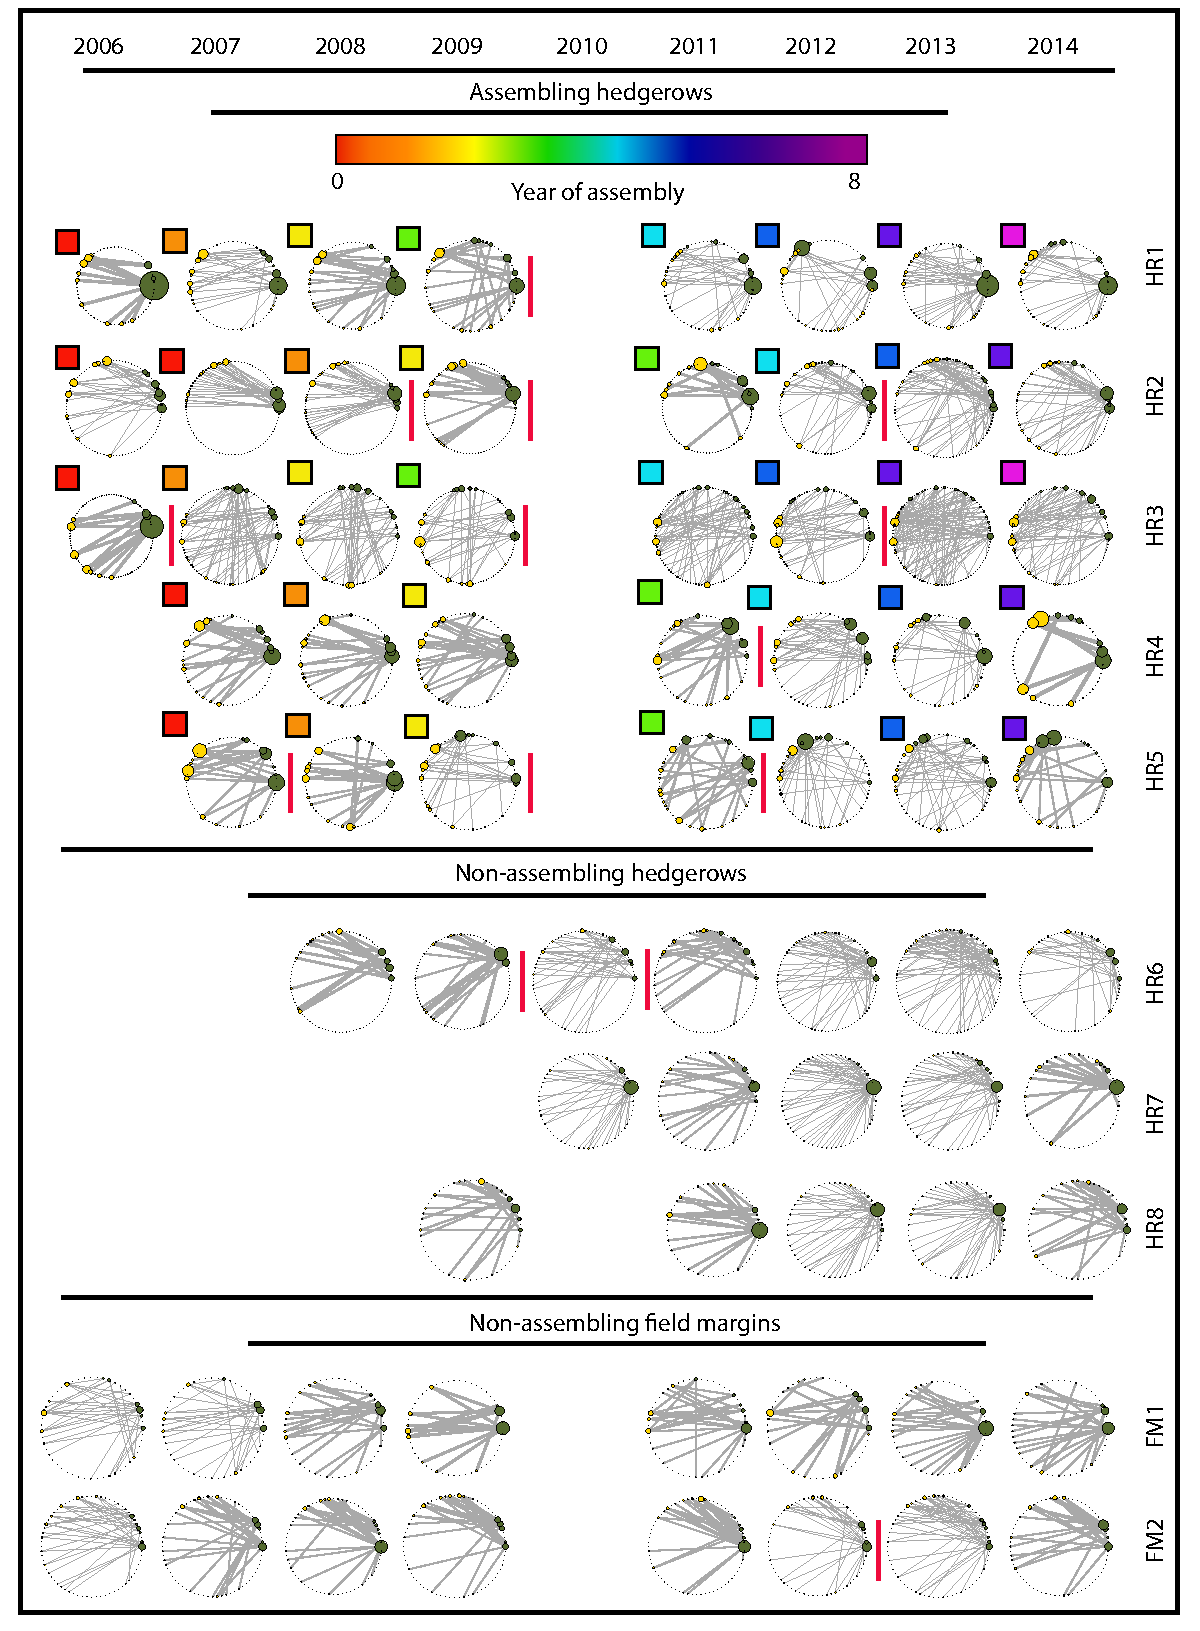
\includegraphics[width=.8\textwidth]{../analysis/changePoint/plotting/networks.pdf}
  \caption{\DIFdelbeginFL \DIFdelFL{The network structure and changing points (vertical red
    lines) in assembling hedgerows and a representative sample of
    non-assembling hedgerows and weedy field margins. In each network,
    plants and pollinators are represented by green and yellow
    circles, respectively, weighted by their degree. Each species has
    has a consistent position in the network across years. In the
    assembling hedgerows, colored circles in the corner of each
    network represent the years post restoration.}\DIFdelendFL \DIFaddbeginFL \DIFaddFL{XXX}\DIFaddendFL }
  \label{fig:changePoints}
\end{figure}
\clearpage

\subsubsection*{Characteristics of \DIFdelbegin \DIFdel{species that contribute to change
  points}\DIFdelend \DIFaddbegin \DIFadd{``core'' and ``peripheral''
  communities}\DIFaddend }


\DIFdelbegin \DIFdel{In contradiction to the predictions of assembly by preferential
attachment, both pollinator persistence and degree were positively
related to network position variability. (ADD STATS IF KEEPING
RESULT).
}\DIFdelend %DIF > Maybe use the same color to all peripheral species communities? Are they giving us any extra information?
\DIFaddbegin \begin{figure}
  \centering
  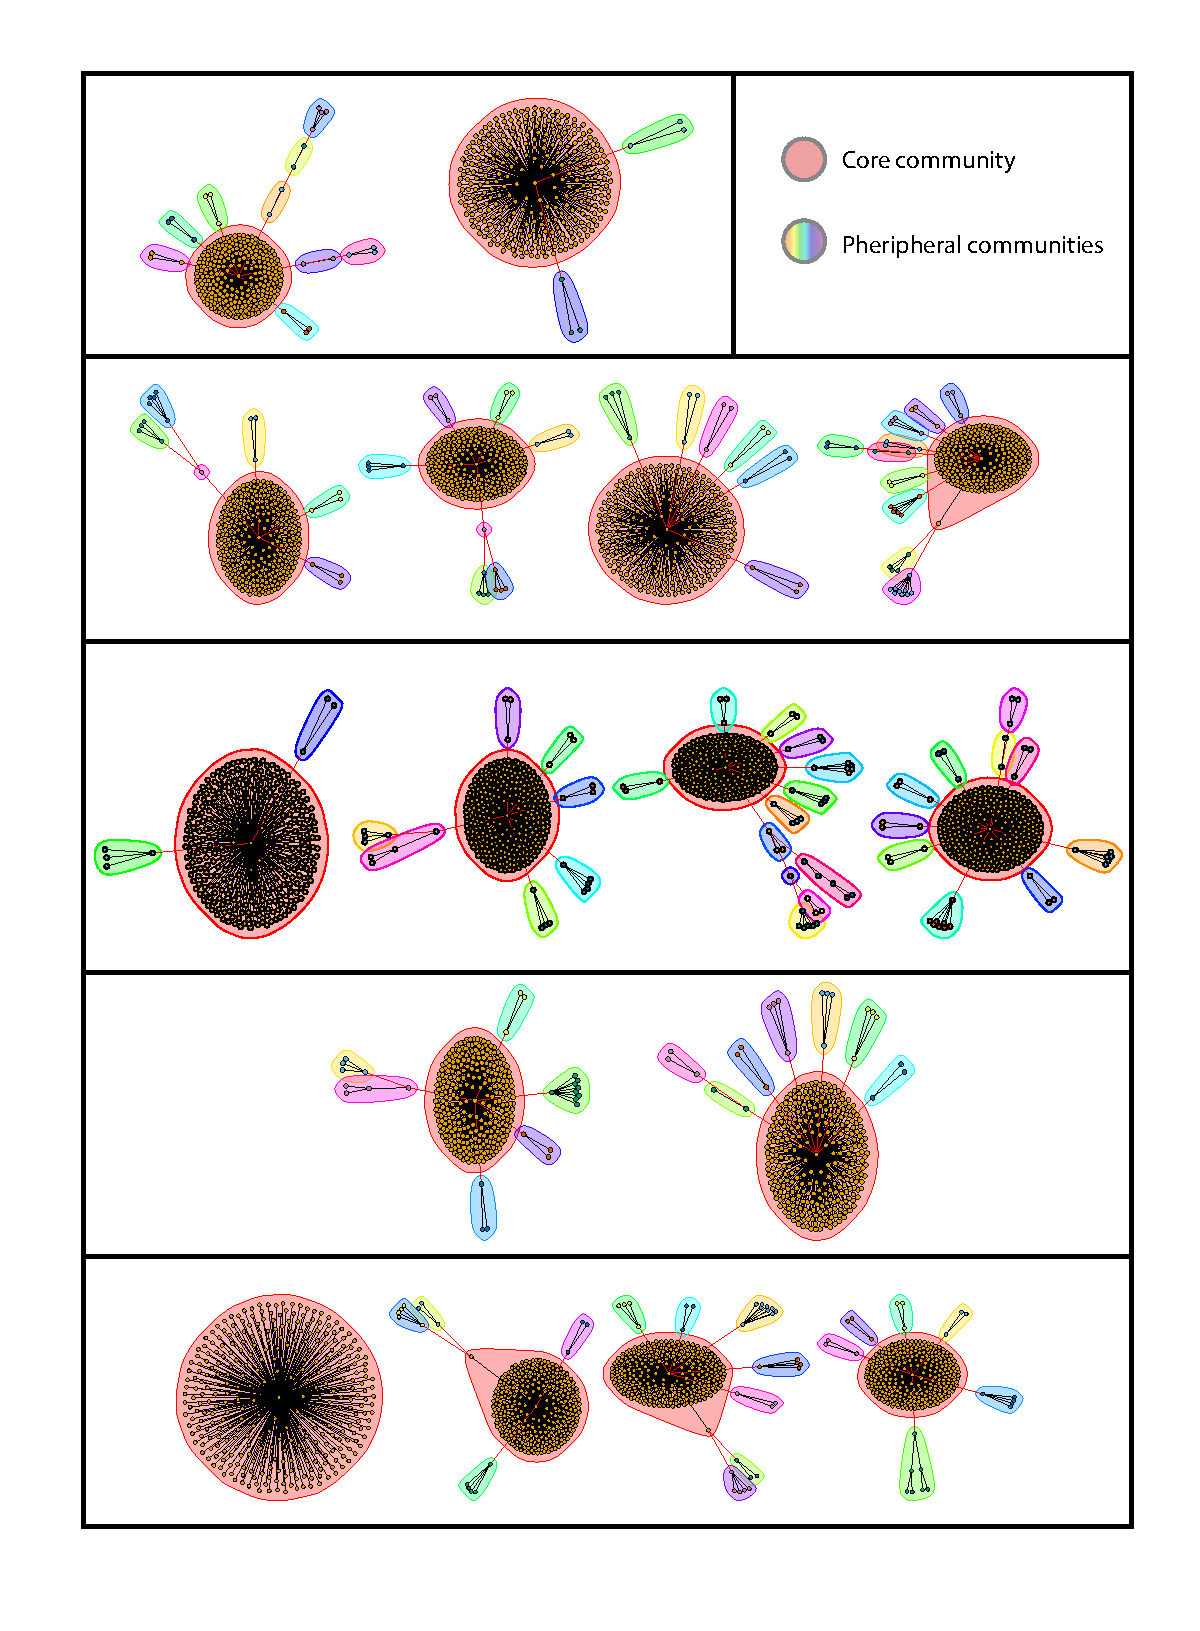
\includegraphics[width=.8\textwidth]{../analysis/changePoint/plotting/communities.pdf}
  \caption{\DIFaddFL{XXX}}
  \label{fig:communities}
\end{figure}
\clearpage
\DIFaddend 

\begin{figure}
  \centering
  \DIFdelbeginFL %DIFDELCMD < 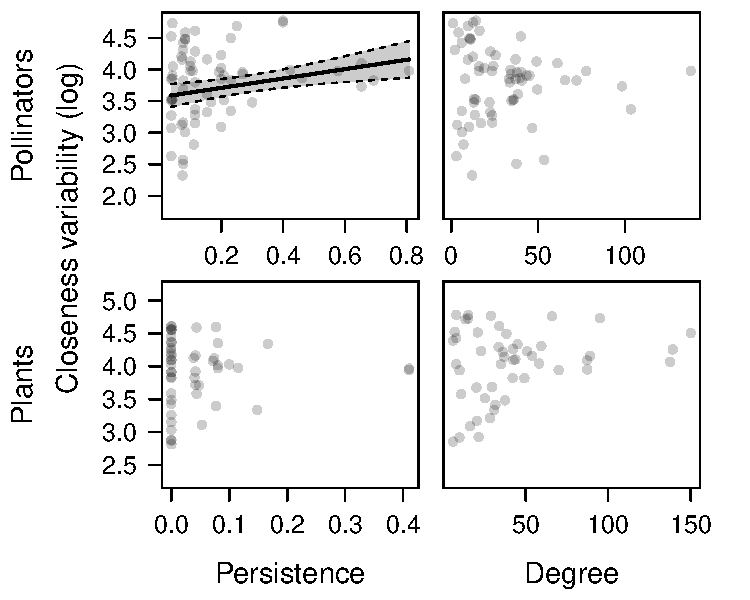
\includegraphics[width=.8\textwidth]{../analysis/variability/figures/cv/occ_degree.pdf}
%DIFDELCMD <   %%%
\DIFdelendFL \DIFaddbeginFL 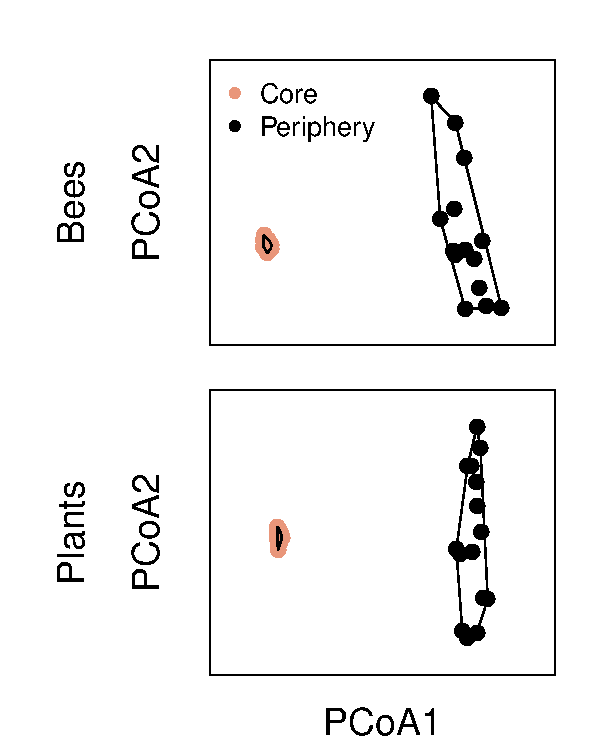
\includegraphics[width=.7\textwidth]{../analysis/changePoint/plotting/figures/pcoa/pcoa.pdf}
  \DIFaddendFL \caption{\DIFdelbeginFL \DIFdelFL{The coefficient of variation of network position, as
    represented by closeness, plotted against pollinator persistence
    and degree. Points represents means for each species across sites.
    The solid line indicates the mean slope estimate and the dashed
    lines are the $95\%$ confidence intervals around the estimate. }\DIFdelendFL \DIFaddbeginFL \DIFaddFL{XXX}\DIFaddendFL }
  \DIFdelbeginFL %DIFDELCMD < \label{fig:cv}
%DIFDELCMD < %%%
\DIFdelendFL \DIFaddbeginFL \label{fig:pcoa}
\DIFaddendFL \end{figure}
\clearpage

\DIFdelbegin \section*{\DIFdel{Temporal changes in interaction patterns}}
%DIFAUXCMD
\DIFdelend \subsection*{Network structure}
\DIFdelbegin \DIFdel{Network nestedness significantly increased with assembly (estimate of
the slope of nestedness through time $\pm$ standard error of the
estimate, $1.834 \pm 0.6142$, $p$-value=$0.022$, Fig.~
\ref{fig:baci}).  Modularity decreased (Fig.~ \ref{fig:baci}), though
the slope was not significantly different from zero (estimate of the
slope of modularity through time $\pm$ standard error of the estimate,
$-0.524$ $\pm$ $0.295$, $p$-value=$0.124$). Specialization remained
relatively constant (estimate of the slope of specialization through time
$\pm$ standard error of the estimate, $0.003$ $\pm$ $0.015$,
$p$-value=$0.827$).
}\DIFdelend 

\begin{figure}
  \centering
  \DIFdelbeginFL %DIFDELCMD < 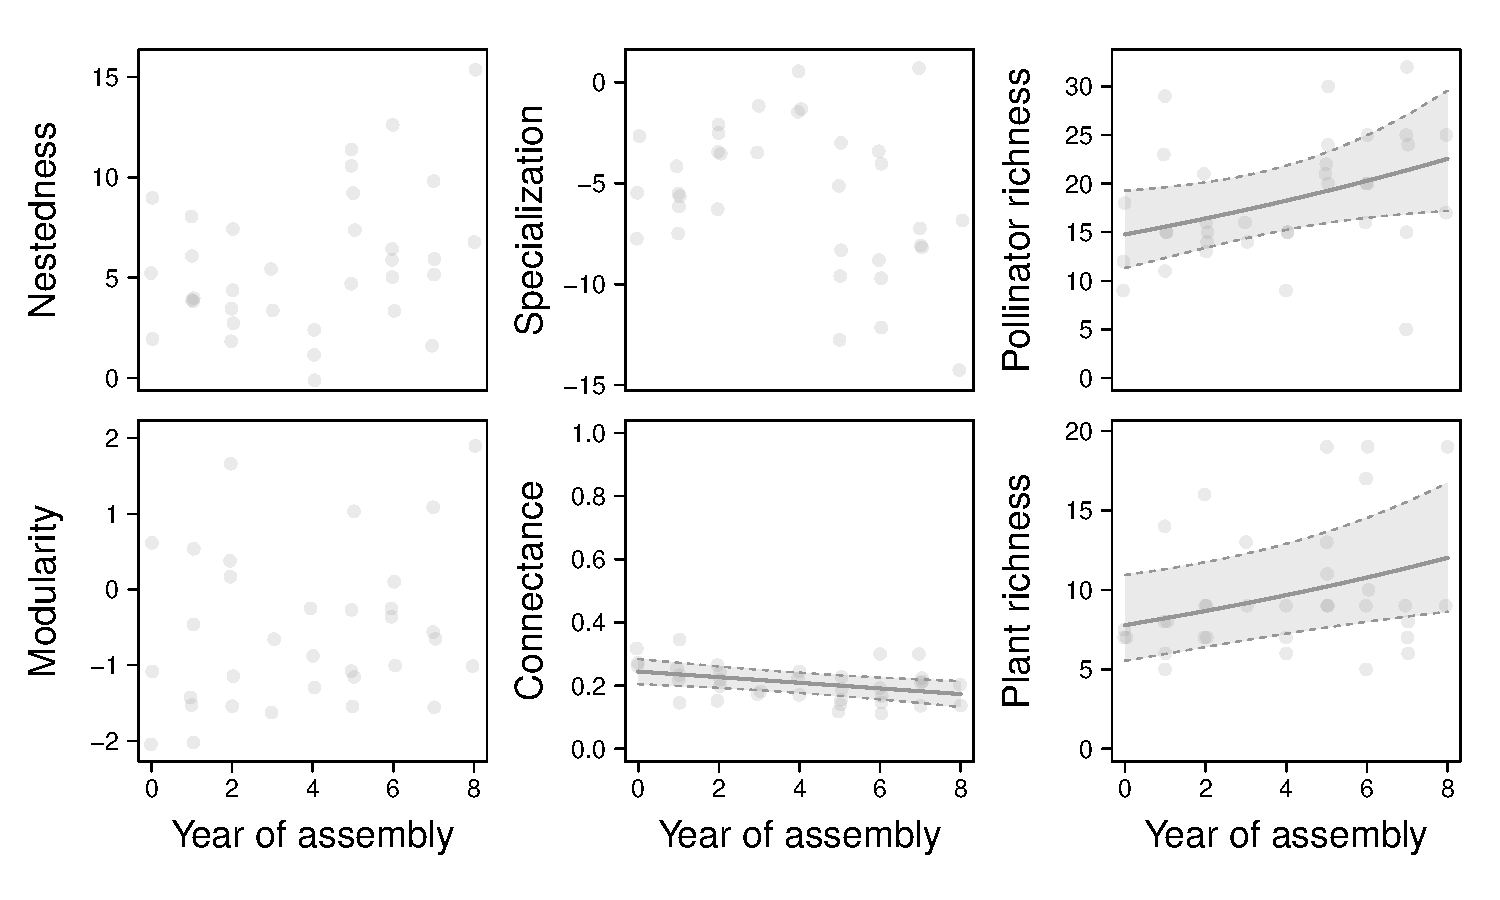
\includegraphics[width=.7\textwidth]{../analysis/networkLevel/figures/baci.pdf}
%DIFDELCMD <   %%%
\DIFdelendFL \DIFaddbeginFL 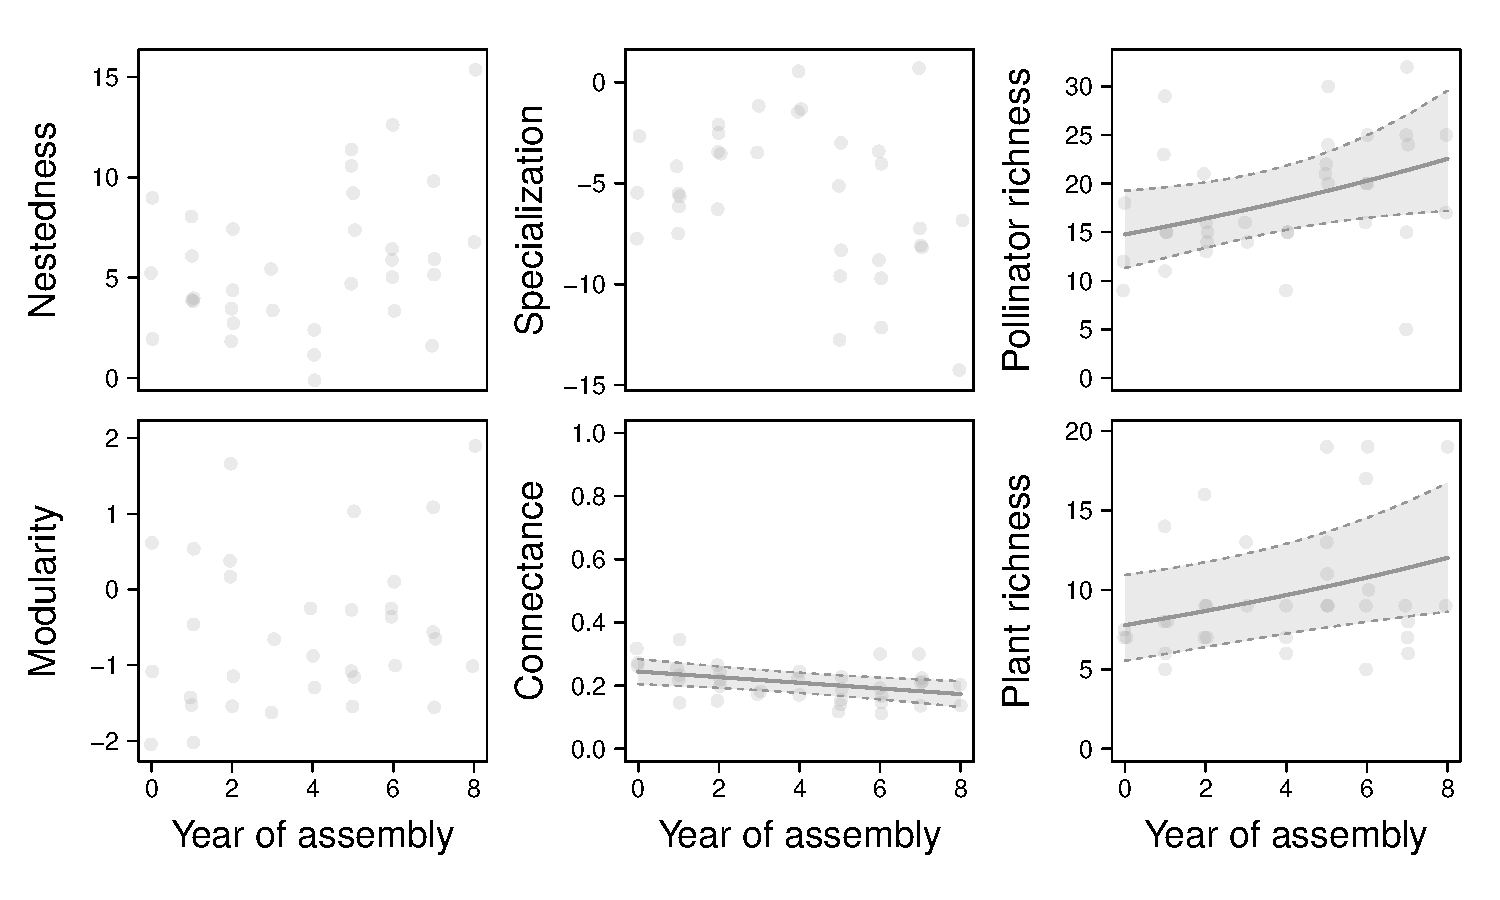
\includegraphics[width=.4\textwidth]{../analysis/networkLevel/figures/baci.pdf}
  \DIFaddendFL \caption{\DIFdelbeginFL \DIFdelFL{The change in nestedness, modularity, specialization and
    connectance as the networks assemble. The left panels represent
    $z$-scores. Scores greater than $\sim 2$ or less than $\sim -2$
    are significantly more or less structured than randomly assembled
    networks. Points are the value for each site at each year of
    assembly. The solid line indicates the mean slope estimate and the
    dashed lines are the $95\%$ confidence intervals around the
    estimate.}\DIFdelendFL \DIFaddbeginFL \DIFaddFL{XXX}\DIFaddendFL }
  \label{fig:baci}
\end{figure}
\clearpage

\subsection*{Network robustness}
\DIFdelbegin \DIFdel{Assembly did not effect the robustness of the networks to species
extinction when species where removed incrementally by degree
(estimate of the slope of robustness through time $\pm$ standard error
of the estimate, $6*10^{-5} \pm 4*10^{-3}$, $p$-value=$0.987$) or
abundance ($0.001 \pm 0.003$, $p$-value=$0.65$, Fig.~ \ref{fig:rob}).
}\DIFdelend 

\DIFdelbegin \DIFdel{In contrast, the robustness of networks to perturbation, as measured
by the algebraic connectivity of the network, increased as the network
assembled (estimate of the slope of robustness through time $\pm$
standard error of the estimate, $0.6814 \pm 0.272$, $p$-value=$0.042$,
Fig.~ \ref{fig:rob}).
}\DIFdelend %DIF > % no need for robustness figs bec not sig

\DIFdelbegin %DIFDELCMD < \begin{figure}
%DIFDELCMD <   \centering
%DIFDELCMD <   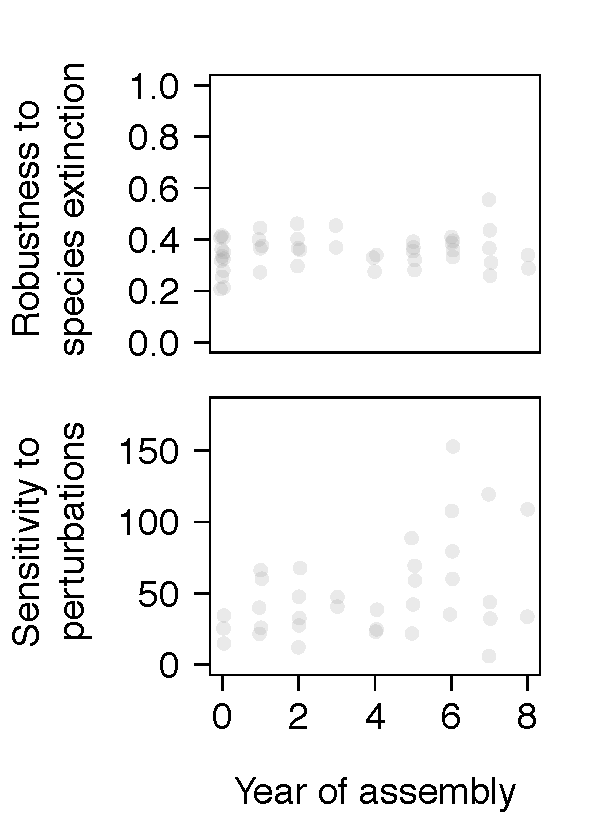
\includegraphics[width=.7\textwidth]{../analysis/networkLevel/figures/robustness.pdf}
%DIFDELCMD <   %%%
%DIFDELCMD < \caption{%
{%DIFAUXCMD
\DIFdelFL{The robustness of networks to species extinction and
    perturbation. The robustness to species extinction is measured by
    incrementally removing species by degree, through removing
    species by abundance did not yield qualitatively different
    results. Points are the value for each site at each year of
    assembly. The solid line indicates the mean slope estimate and the
    dashed lines are the $95\%$ confidence intervals around the
    estimate.}}
  %DIFAUXCMD
%DIFDELCMD < \label{fig:rob}
%DIFDELCMD < \end{figure}
%DIFDELCMD < \clearpage
%DIFDELCMD < 

%DIFDELCMD < %%%
\DIFdelend \section*{Discussion}
\label{sec:discussion}

\section*{Acknowledgments}
\label{sec:acknowledge}

%DIF >  I think we should thank SF and CSSS somehow... 
We would like to thank Leto Peel and Aaron Clauset for their
invaluable discussions and for help with the change point analysis.
We thank the growers and land owners that allowed us to work on their
property.  We also \DIFdelbegin \DIFdel{greatly }\DIFdelend appreciate the identification assistance of expert
taxonomists Martin Hauser, Robbin Thorp and Jason Gibbs.  This work
was supported by funding from the Army Research Office
(W911NF-11-1-0361 to CK), the Natural Resources Conservation Service
(CIG-69-3A75-12-253, CIG-69-3A75-9-142, CIG-68-9104-6-101 and
WLF-69-7482-6-277 to The Xerces Society), the National Science
Foundation (DEB-0919128 to CK), The U.S.  Department of Agriculture
(USDA-NIFA 2012-51181-20105 to Michigan State University).  Funding
for LCP was provided by an NSF Graduate Research Fellowship and the
USDA NIFA Graduate Fellowship. \DIFdelbegin \DIFdel{FUNDING FOR MARILLIA}\DIFdelend \DIFaddbegin \DIFadd{Funding for MPG was provided by Sao Paulo Research Foundation (FAPESP, grant 2013/13319-5)}\DIFaddend .

\bibliographystyle{ecol_let}

\bibliography{refs}
\DIFdelbegin %DIFDELCMD < 

%DIFDELCMD < %%%
%DIF <  \subsection*{Core and peripherial communities}
%DIFDELCMD < 

%DIFDELCMD < %%%
%DIF <  To classify species as we first generate dendrograms using the GHRG
%DIF <  model before and after each change point.  We then determined which
%DIF <  species belonged to the ``core'' and ``peripheral'' network
%DIF <  communities at each site. The ``core'' network communities contain the
%DIF <  majority of species and are more basil than the more derived, less
%DIF <  specious ``peripheral'' network communities. We next use a
%DIF <  Permutational Multivariate Analysis of Variance (PERMANOVA)
%DIF <  \citep{anderson-2013-557} to determine whether the species
%DIF <  compositions of the species that belonged to the core and peripheral
%DIF <  communities differed. We also test whether core or peripheral species
%DIF <  had more variability in their species compositions \citep[i.e.,
%DIF <  multivariate dispersion][]{anderson-2011-19, anderson-2006-683}.
%DIFDELCMD < 

%DIFDELCMD < %%%
%DIF <  Lastly, we explored the functional diversity of the core and
%DIF <  peripheral pollinator species
%DIFDELCMD < 

%DIFDELCMD < %%%
%DIF <  The syrphids in our study area have similar traits, so we focused on
%DIF <  the trait diversity of the bee subset of our interaction networks. We
%DIF <  focus on resource capture and use traits that collectively
%DIF <  \citep{kremen-2015-602} including resource specialization
%DIF <  \citep[quantitative, $d'$;][]{bluthgen-2006-9}, body size
%DIF <  \citep[quantitative, inter-tegular span, mm,][]{cane-1987-145},
%DIF <  sociality (categorical: eusocial, solitary, cleptoparasitic), nest
%DIF <  location (categorical: above ground, below ground or mix), and nest
%DIF <  construction \citep[categorical: excavator, mason or
%DIF <  renter;][]{williams-2010-2280} as described in more detail in
%DIF <  \cite{kremen-2015-602}.  Each trait has the same weight in trait
%DIF <  diversity metric estimation \citep{villeger-2008-2290,
%DIF <  schleuter-2010-469}.
%DIFDELCMD < 

%DIFDELCMD < %%%
%DIF <  To characterize the functional diversity of the bee species in core
%DIF <  and peripherial communities, we computed three metrics that capture
%DIF <  diversity, uniqueness, and distribution of functional values in the
%DIF <  community: functional dispersion, divergence, and evenness
%DIF <  \citep{villeger-2008-2290, schleuter-2010-469}.  Functional
%DIF <  dispersion is a measure of trait diversity, corrected for species
%DIF <  richness \citep{schleuter-2010-469}; functional divergence measures
%DIF <  how species abundances are distributed within the trait space
%DIF <  \citep[i.e., a measure of functional
%DIF <  uniqueness,][]{villeger-2008-2290}; functional evenness measures the
%DIF <  regularity with which traits are distributed across functional
%DIF <  space, accounting for abundance \citep{villeger-2008-2290}.  In
%DIF <  combination, these metrics provide a relatively complete overview of
%DIF <  the different aspects of functional diversity
%DIF <  \citep{villeger-2008-2290, schleuter-2010-469}. To determine whether
%DIF <  trait evenness, dispersion, and divergence differed between controls
%DIF <  and hedgerows at different stages of maturation, we used the trait
%DIF <  diversity metrics as response variables in linear mixed models with
%DIF <  site type as a fixed effect and year and site as random effects
%DIF <  \citep{lme4,lmetest}.
\DIFdelend 


\end{document}

%%% Local Variables:
%%% mode: latex
%%% TeX-PDF-mode: t
%%% End:
